\chapter{Analysis and Discussion of Model Results} % (fold)
\label{cha:analysis_of_model_results}
In the study of evolutionary dynamics there exists the concept of a stable equilibrium. The organisms in such a situation may not all represent the ``best fit'' mechanism for coping with a particular ecological niche, but at the same time none are sufficiently better off than the others that they will dominate the population. If organisms polymerizing nucleotides in a $3'\to5'$ direction represented a stable equilibrium with organisms polymerizing in a $5'\to3'$ direction, then it would be expected that organisms exhibiting such a trait should be found in nature. On the other hand, if $3'\to5'$ polymerization is a loosing strategy when in competition with $5'\to3'$ polymerization, the lack of modern $3'\to5'$ polymerizing organisms would be an expected consequence of Darwinian evolution.

When modeling the competition between organisms with a $5'\to3'$ polymerase and organisms with a $3'\to5'$ polymerase, this is an important aspect of modern evolutionary theory to keep in mind. It is not sufficient to show that polymerizing nucleotides in a $5'\to3'$ direction is better fit than, or produces organisms which reproduce faster than polymerizing nucleotides in a $3'\to5'$ direction. Rather, to discriminate between the possibility that the modern ubiquity of $5'\to3'$ polymerases is the result of a founder effect versus being a consequence of natural selection, we need to show that $3'\to5'$ polymerizing organisms cannot exist in a stable equilibrium. It is with this in mind that the model presented here was constructed.

In constructing this model, a number of explicit and implicit assumptions were made. The first, and perhaps largest, assumption is that polymerizing nucleotides to create new nucleic acid polymers by adding nucleotide triphosphates to the $5'$ end of the growing chain is physically possible. As there are no known polymerase enzymes which carry out the polymerization reaction in a $3'\to5'$ direction, it is impossible to say with certainty that such polymerases might exist. However, based on the nature of the active site chemistry of nucleotide polymerases, there is also no reason to believe that such $3'\to5'$ polymerases are not possible, beyond the fact that such polymerases do not currently exist. For this reason, we are comfortable with this assumption.

The second implicit assumption made in constructing this model is that the only viable building blocks for nucleic acid polymers are $5'$-triphosphate nucleotides. If nucleotides phosphorylated on their $3'$ oxygen could be used by a hypothetical $3'\to5'$ polymerase, then the chemistry of such a polymerase would not, qualitatively, be any different than that of a $5'\to3'$ polymerase working with $5'$-triphosphate nucleotides. That is, in the case that a $3'\to5'$ polymerase could work with a $3'$-triphosphate nucleotide, then the activated triphosphate moiety would reside on the incoming nucleotide, instead of on the growing chain, in the same way that the triphosphate moiety is found on the incoming $5'$-triphosphate nucleotide used by $5'\to3'$ polymerases.

We can discount the possibility of $3'$-triphosphate nucleotides as raw material for a polymerase reaction for a number of reasons. If, in keeping with current scientific consensus, ribonucleic acids represent the more ancient form of nucleotides and the $2'$-deoxyribonucleic acids are a more recent invention of biology, then a potential $3'$-triphosphate nucleotide would have its triphosphate group attached on a carbon adjacent to a free hydroxyl. The free $2'$-hydroxyl group of ribonucleic acids is known to polymerize hydrolysis reactions in a number of ribozymes, so it would not be unreasonable to assume that the $2'$-hydroxyl would also catalyze a hydrolysis of the triphosphate group on a $3'$-triphosphate nucleotide. This would serve to significantly restrict the available primordial pool of $3'$-triphosphate nucleotides as compared to $5'$-triphosphate nucleotides, whose adjacent carbon's oxygen would normally be incorporated in the formation of the furanose ring. Indeed, it has been shown that ribose-$3'$-phosphate decomposes more readily under mild acid conditions than ribose-$5'$-phosphate.

The remaining assumptions made are the various explicit assumptions required for construction of the model itself as described in chapter~\ref{cha:design_of_the_polymerase_evolution_model}. Of these, the most important is the assumption that the dynamics of spontaneous nucleotide hydrolysis occur on a time-scale commiserate with the time-scale of nucleotide incorporation and the assumption of a geometry-based discrimination mechanism for incorrect nucleotide incorporation by the polymerase. We can surmise that the time-scale for spontaneous nucleotide hydrolysis cannot be significantly smaller than the time-scale for nucleotide incorporation, for if it were then nucleotide polymerization would, in effect, be impossible. If the time-scale were much larger, this would be the equivalent of removing a constant factor from the calculation for the probability that nucleotide inactivation occurs during polymerization. The effect of such an adjustment would be largely quantitative, raising the simulation temperature at which the effects reported would be observed.

A note should be made on the significance of the simulation temperature used in the model. If we take the expression used in the model for the temperature dependence of the equilibrium between the polymerase-template-nucleotide complex for the correct nucleotide, the free polymerase-template complex, and the polymerase-template-nucleotide complex for the incorrect nucleotide: $e^{-\frac{1}{t}}$, and compare it to the experimentally determined value of $5 \frac{kcal}{mol}$ for the $\Delta\Delta G$ of this system, we can calculate the real temperature corresponding to each simulation temperature with the expression\[
	T = t \frac{5\frac{kcal}{mol}}{R}
\]
This gives us a real temperature of $-22^\circ \rm{C}$ for a simulation temperature of 0.10 and a real temperature of $1200^\circ \rm{C}$ for a simulation temperature of 0.60. Obviously this range of temperatures is unreasonably large for life, even when accounting for aqueous environments with high salinity or at high pressures.

As mentioned in the introduction, every effort was made when designing this model to remain faithful to the realities of the biochemical processes that a nucleotide polymerase must carry out. That said, a number of confounding factors limit the applicability of the precise quantitative temperature values used in the simulations to understanding real biological processes. It has already been mentioned that the need to reduce the probability of spontaneous nucleotide hydrolysis by a constant factor to account for a difference in time-scales would effect the absolute temperature values at which various simulation outcomes are observed. The same sort of constant factor consideration would, potentially, also need to be made to account for a difference between the precise effect of geometry-based discrimination of real nucleotide polymerases and the model values.

The primary model values impacted by simulation temperature are those for the equilibrium describing the incorporation of correct versus incorrect nucleotides during nucleic acid synthesis, and the equilibrium between active and inactive nucleotides. The chemical phenomena described by these values, however, are subject to more influences than just temperature. For example, it is well documented that the energy associated with a correct nucleotide base-pairing is heavily influenced by the dielectric constant of the solvent and the concentration of nucleic acid counter-ions. The equilibrium of nucleotide triphosphates would, likewise, be subject to influence by effects of nucleotide concentration and pH. Thus, the value of simulation temperature can be thought of as a stand in for a number of thermodynamic factors that might influence the biochemical processes involved in the model processes. Therefore, the primary utility of the simulation temperature is in revealing the collected influence of thermodynamics on the system. Before we consider these influences, let us look at the results of the initial experiments performed with the model.


\subsubsection*{Effect of Temperature on Evolution}
In constructing the model presented here, we were attempting to evaluate the plausibility of the hypothesis that all life contains nucleotide polymerases which proceed in a $5'\to3'$ direction due to an evolutionary advantage of this mechanism versus the reverse $3'\to5'$ direction. In order to address this question while still remaining biologically relevant, it was necessary to account for a pair of temperature dependent chemical processes: spontaneous hydrolysis of nucleotide triphosphates and inclusion error rate.

First, to validate the kinetics of the model we carried out a number of simulations in which each sort of organism, those containing the $5'\to3'$ (forward) polymerase and those containing the $3'\to5'$ (reverse) polymerase, were allowed to grow from a small starting population in the absence of competition (fig.~\ref{fig:temp_incr_mut}\textbf{A}). These experiments revealed that the temperature of the environment had a gradual impact on the growth rate of the model organisms, with the greatest inhibition on growth rate occurring at the highest temperatures investigated. At these higher temperatures, the effect on growth appeared to be greater on organisms containing the reverse polymerase than on those containing the forward polymerase. This indicates that the disadvantages inherent in polymerizing nucleic acids in a $3'\to5'$ direction become more exaggerated as the temperature increases.

Another way to analyze these experiments is to look at the way that the rate of the nucleotide polymerases evolves at each temperature. Generally, we can state that tendency toward a faster polymerase indicates that the predominant evolutionary pressure is on reproduction rate, while a tendency toward slower polymerases indicates an increased importance of reducing the mutation rate. This stems from the fact that a faster polymerase will have a greater error rate. With this in mind, figure~\ref{fig:temp_incr_mut}\textbf{B} shows that, as the temperature of the simulation increases, the average polymerase rate decreases indicating the increasing importance of avoiding errors. This is true up to simulation temperatures of 0.40, but at a simulation temperature of 0.60 the trend reverses indicating a switch back toward reproduction rate as the primary evolutionary pressure.

This switch most likely represents a saturation of the effect that mutation can have on the organisms. That is, in our model system an increasing mutation rate decreases the fidelity with which each generation can pass along its traits (in this case just polymerase rate) to subsequent generations. We expect that, at some high mutation rate, this fidelity drops significantly enough that the polymerase rate inherited from one generation to the next is not significantly distinguishable from a randomly assigned value. When the temperature of the simulation gets high enough, the error rate due to the thermal component will overwhelm the error rate due to polymerase rate, and reach this critical value. At this point the selective pressure against faster polymerases resulting from the need to preserve generation to generation fidelity will, in effect, vanish. In our system, this leaves growth rate as the single remaining selective pressure, explaining the reversal of the trend of polymerase rate evolution at high simulation temperatures. Indeed, as can be seen in figure~\ref{fig:mut_rate}, at simulation temperatures of 0.55 and 0.60, the average change in polymerase rate from one generation to the next is nearly 5, the maximum that would be expected if polymerase rates were inherited at random.

\begin{figure}[!ht]
	\begin{center}
		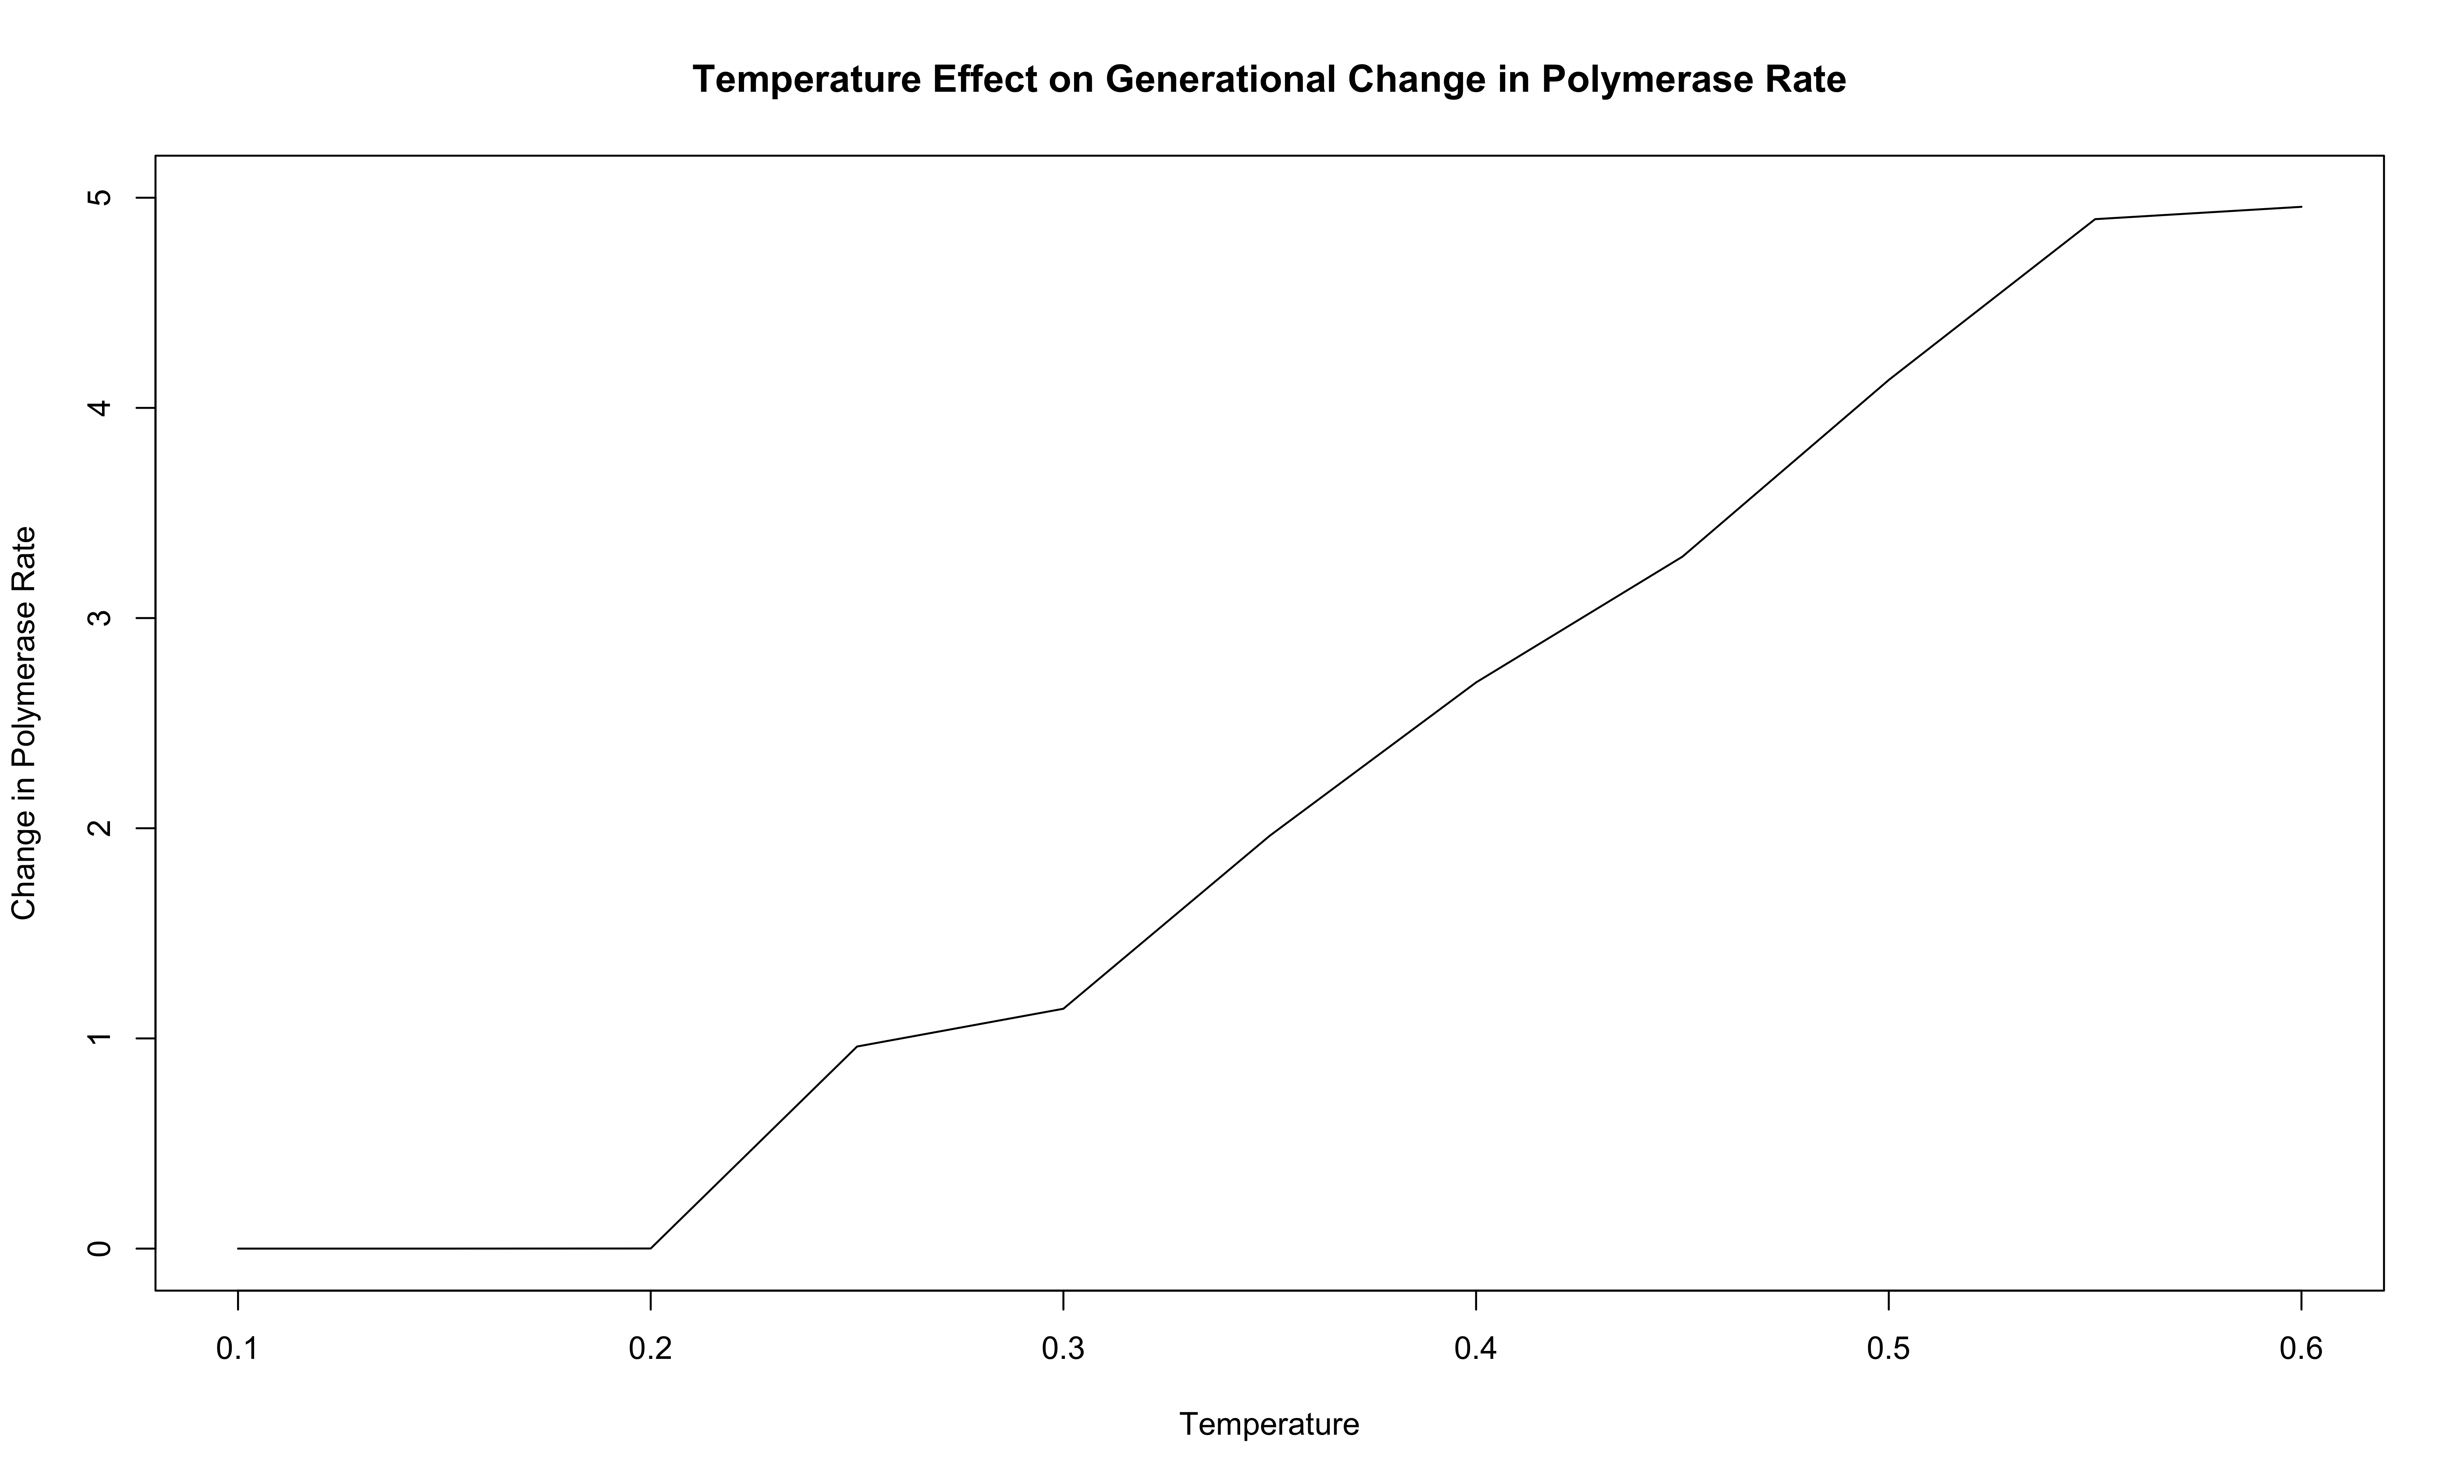
\includegraphics[width=\textwidth]{mutation_rate}
	\end{center}
	\caption{
		{\bf Generational change in polymerase rate as a function of temperature.}  The organisms from the systems plotted in \ref{fig:temp_incr_mut} were analyzed for the difference between the rate of their polymerase and the rate of their parent's polymerase. This difference is plotted for the various different temperatures simulated. The maximal difference we would expect to see (i.e. in the case that inheritance was purely random) would be 5.
		}
		\label{fig:mut_rate}
\end{figure}

One interesting result from this first experiment that was not completely anticipated was that the polymerase rate of the forward and reverse polymerizing organisms would be so similar over a wide range of simulation temperatures. We expected that reverse polymerizing organisms, with the increased penalty for a spontaneous hydrolysis event, would have a greater selective pressure to evolve a faster polymerase holding all else constant. This seems to not be the case, though, as the average polymerase rate of the forward and reverse polymerizing organisms at all but the highest temperature are indistinguishable. The only conclusion we can draw from this observation is that the selective pressure on mutation rate is sufficiently rigid enough to make the spontaneous hydrolysis penalty a negligible influence on the evolution of polymerase rate. This conclusion is further backed up by evidence from the simulations with no mutation allowed, as described below.

The next set of experiments was intended to look at how forward and reverse polymerizing organisms would fare in competition with each other at various temperatures. We again started each simulation with a small seed population and allowed these populations to grow in an exponential fashion. As we expected based on the similarity of growth rates for the forward and reverse polymerizing organisms growing in isolation, both forms grew rapidly until the environment was at capacity with approximately half of the population belonging to each form. At this point, competition kicks in and at simulation temperatures of 0.1 an equilibrium between the two forms is established. At a simulation temperature of 0.3, it is unclear in the duration of the simulation run whether an equilibrium might eventually be established or whether the reverse polymerizing organisms would eventually be outcompeted. At the higher simulation temperatures of 0.4 and 0.6, the reverse polymerizing organisms are outcompeted by the forward polymerizing forms, however at the temperature of 0.4 this is a true out-competition, where the reverse polymerizing form grew to occupy nearly half the population before being eradicated. At a simulation temperature of 0.6, the reverse polymerizing organisms are never able to establish themselves.

At the higher temperatures, the average polymerase rate of the reverse polymerizing organisms begins to drop off as their population numbers, as seen in figure~\ref{fig:growth_compet_mut}\textbf{B}, begin to drop off. This drop is not, however, indicative of a reduction in the fitness of the reverse polymerizing organisms. Rather, as the reverse polymerizing organisms are gradually outcompeted by the forward polymerizing organisms their number is reduced. Since the only mechanism in the model for removing organisms from the population is the density dependent random culling, which members of the reverse polymerizing organism population will be removed is likewise random. Since the organisms with a faster polymerase rate will reproduce more rapidly, they will be present in greater number, and therefore will be more likely to be removed from the environment first. In other words, the rate of the decrease in average polymerase rate of the reverse polymerizing organisms can be seen as a proxy measure for the rate at which the forward polymerizing organisms are preferentially occupying the available capacity in the environment created when a reverse polymerizing organism is culled.

Looking at the evolution of the polymerase rates of the forward and reverse polymerizing organisms, it is apparent that the selective pressure on polymerase rate is greater when there is competition involved at low temperatures. That is, at a simulation temperatures of 0.3 and 0.4, the steady-state polymerase rate under competition is not appreciably different than under the no competition growth case, but at a simulation temperature of 0.1 the steady-state polymerase rate under competition is elevated as compared to the average polymerase rate for both forward and reverse polymerizing organisms growing in isolation. From this we can conclude that rapid growth takes on an increased importance when competition with an alternative strategy is involved.

Because the reverse polymerizing organisms were not able to grow significantly at a temperature of 0.6 under competition, and because of the ambiguity of the eventual fate of the reverse polymerizing organisms at a temperature of 0.3, we were curious what might happen if both forms started off at a significantly larger population size. Specifically, we were interested to see if forward polymerizing organisms represented an evolutionarily stable strategy at these temperatures\cite[chap. 4]{ANowak:2006p857}. In order to investigate this question, we carried out simulations starting with completely full environments split evenly between forward and reverse polymerizing organisms at various temperatures.

The results from these simulations (fig.~\ref{fig:strict_compet_mut}) indicate that the ultimate success of the forward and reverse strategies in competition with each other when starting from half of an environment at capacity is similar to that during exponential growth, though the dynamics are interestingly different. In general, we can conclude that forward and reverse polymerizing organisms will establish an equilibrium at lower temperatures and that forward polymerizing organisms are dominant at higher temperatures. That is, at sufficiently high enough temperatures, polymerizing nucleotides in a $5'\to3'$ direction appears to be an evolutionarily stable strategy.

Also, the steady state polymerase rates reached at each temperature are the same as for the exponential growth case above. The simulations starting with a full population differ from those starting with exponentially growing populations in how the steady state is reached. Arrival at the steady state polymerase rate occurs much earlier in the case of exponential growth. This reflects the fact that in a mostly empty environment it is easier for the best fit organisms to rapidly dominate a population. In a population already at capacity, this rebalancing of traits can only occur through attrition, which is a more gradual process. Interestingly, the rate at which the steady state polymerase rate is achieved appears to impact the distribution of the equilibrium population. At a simulation temperature of 0.1, the equilibrium population in the exponential growth case is evenly divided between forward and reverse polymerizing organisms, but in the full environment case the split is closer to $\frac{3}{4}$ forward polymerizing organisms and $\frac{1}{4}$ reverse. We believe that this difference may point toward the existence of different domains of competition. That is, it may be possible that the fitness of the model organisms is impacted by the population relative to the environment's carrying capacity. Since there are two fitness components encoded in the polymerases of our model organisms, namely proliferation rate and mutation rate, what we may be observing is the existence of multiple fitness equilibria between the forward and reverse polymerizing organisms. Future models wherein these fitness components could be decoupled might help resolve this possibility.


\subsubsection*{Effect of Mutation on Evolution}
To better understand the role that mutation and the introduction of random variation from generation to generation might have on the results of our simulations, we modified the model system to remove the possibility for mutation. With this modification, the average polymerase rate can still evolve, but only through selection of individuals. Also, since the only evolutionary pressure acting on the model organisms is reproduction rate, we would expect that all individuals should converge on the maximum polymerase rate. Indeed, this is precisely the result we observe (fig.~\ref{fig:temp_incr_nomut}\textbf{B}). With the selective pressure of mutation removed, we can also directly observe the impact of the penalty on reverse polymerizing organisms due to spontaneous hydrolysis of nucleotide triphosphates. In figure~\ref{fig:temp_incr_nomut}\textbf{B}, we can see that at simulation temperatures of 0.4 and 0.6 the reverse polymerizing organisms evolve to faster polymerase rates sooner than their forward polymerizing counterparts.

We also note that the exponential growth of both the forward and reverse polymerizing organisms is essentially identical at all temperatures except for 0.6 (fig. ~\ref{fig:temp_incr_nomut}\textbf{A}). Reverse polymerizing organisms at a simulation temperature of 0.6 are the only group to deviate. This is due to the excessive penalty paid by a reverse polymerase at this high temperature. Moreover, the reverse polymerizing organisms at a simulation temperature of 0.4 appear to grow with identical kinetics to the forward polymerizing organisms at this temperature, showing that the penalty of a reverse polymerizing strategy can be compensated for by evolving a faster polymerase (as seen in fig.~\ref{fig:temp_incr_nomut}\textbf{B}).

Following this initial result, we then repeated the prior experiments starting with small populations and starting with a full environment, but with mutations disallowed (figures~\ref{fig:growth_compet_nomut} \&~\ref{fig:strict_compet_nomut}, respectively). When we start with small populations we see, as before, that polymerase rate rapidly evolves to its equilibrium value (fig.~\ref{fig:growth_compet_nomut}\textbf{B}). The difference here is that without mutation this equilibrium value at all temperatures is the maximum polymerase rate allowed. At the highest temperature of 0.6, the reverse polymerizing organisms are unable to establish themselves the same as when mutations were allowed, implying that this inability to compete with forward polymerizing organisms during exponential growth is a consequence of the spontaneous hydrolysis penalty and is not affected by the presence or absence of mutations in the system.

Paying attention to the way that the competition between forward and reverse polymerizing organisms resolves itself at a simulation temperature of 0.4 when starting with a small population (fig.~\ref{fig:growth_compet_nomut}\textbf{A}), its not entirely clear whether an equilibrium between these forms can be established. If we look for the establishment of an equilibrium when starting with a full environment at the same temperature (fig~\ref{fig:strict_compet_nomut}\textbf{A}), it does appear that the forward polymerizing organisms are outcompeting the reverse polymerizing organisms, but the rate at which this take over happens is definitely slower than when mutations are allowed (fig.~\ref{fig:strict_compet_mut}\textbf{A}).

This leaves a question of whether allowing mutations, which affect the generation to generation inheritance of polymerase rate, allow for a more rapid resolution of the more dominant strategy, or whether the addition of mutation to a reverse polymerase strategy causes this to be a loosing strategy when it otherwise might not be. We noticed that the decline in population of reverse polymerizing organisms when starting from a full environment is roughly exponential, so we plotted the natural log of this number against simulation time in figures~\ref{fig:strict_compet_log}, \textbf{A} \& \textbf{B} for simulations where mutations were allowed in the system or where they were prohibited, respectively. These plots represent the rate of population change in each simulation. By calculating the least squares regressions of these rates and plotting the slope of these regressions versus the temperature (fig.~\ref{fig:strict_compet_log}\textbf{C}), we can see clearly that there is an inflection point for both the mutation allowed and the mutation disallowed situations, but that it occurs at different temperatures.

When an equilibrium between forward and reverse polymerizing organisms is established, we expect the rate of population change to not be significantly different from zero. At low simulation temperatures, this is indeed the case. The inflection of the plots in figure~\ref{fig:strict_compet_log}\textbf{C} represents the point at which forward and reverse polymerizing organisms go from being able to establish an equilibrium to a situation where the forward polymerizing organisms are an evolutionarily stable strategy, and the reverse polymerizing organisms will eventually be eradicated from the environment. That this inflection occurs at different temperatures with or without mutations allowed indicates that there is a range of simulation temperatures where mutation does, in fact, make the difference between a forward polymerizing strategy being evolutionarily stable versus merely being the dominant strategy.


\subsubsection*{Founder Effect or Evolution?}
Finally, returning to our original question of whether the present day situation that finds all organisms polymerizing nucleotide polymers in the same $5'\to3'$ direction is the result of a founder event or a consequence of evolution toward a best fit trait, unfortunately the evidence is equivocal. Here we have presented a model system that could potentially explain how evolution might account for the rise of a single polymerase strategy.

At the same time, we have shown that this strategy can coexist with the alternative under the right conditions. That is, at a high temperature it seems clear that polymerizing nucleotides $5'\to3'$ is clearly favored, and would be selected for fairly rapidly. At lower temperatures evolution leads to a predominance of one form, which would make a founder event resulting in a $5'\to3'$ polymerase more likely than the reverse, but evolution alone cannot explain the convergence to a single polymerase strategy.

Really, our inability to link simulation temperature to an actual environmental temperature with any great confidence makes it so that we must leave it at this. We can state that life originating in proximity to a deep sea hydrothermal vent would be more likely to arrive at a single strategy through evolution than life originating in Darwin's ``warm puddle'', though it is possible that both environments would be either above or below the temperature at which evolution leads to a single polymerase form. While this is the most we can conclude from the evidence presented here, combined with other evidence that the machinery involved in DNA polymerization evolved at least twice independently\cite{Leipe:1999p1040}, the weight of evidence favors the explanation that evolutionary competition was the driving factor in determining the modern strategy of nucleotide synthesis.


\subsubsection*{Significance of Results}
Though the evidence presented may not provide conclusive support for or against our original hypothesis, the system constructed and the results obtained from it do present many lessons and interesting leads for future investigations. This is the first system that we are aware of that combines both modeling of the ``evolutionary short-loop'', where mutation alters the replication mechanism which controls the rate of mutation, and simplified real-world thermodynamics of the biochemical processes involved in life. For this reason, this is also the first time we can look at the direct impact that an environmental factor such as temperature has on evolving systems. This is important for the development of theoretical approaches to evolution which depend on interactions between organisms and their environments.

Finally, the model we constructed allowed us to probe the consequences of mutation on evolution. The role of mutations in evolution has long been debated. On one hand, mutations provide variations which are the fodder of natural selection. On the other hand, mutations reduce the information content passed from generation to generation, thereby reducing the efficiency of selection. Our results indicate that the role of mutations in evolution may be complicated by the nature of the evolving system. At low simulation temperatures, mutations appeared to have little to no effect on evolution and competition between forms. In a middle range of simulation temperatures, mutations are the difference between a strategy being able to successful coexist with another and that strategy being a loosing strategy that is eventually eliminated. Finally, at the highest simulation temperatures, the only difference introduced by mutations is a difference in the rate at which the successful strategy is able to outcompete the alternative. This insight into the role that mutations play will surely be invaluable for future investigations.
% chapter analysis_of_model_results (end)